\documentclass[tikz,border=8pt]{standalone}

\usepackage[T1]{fontenc}
\usepackage[utf8]{inputenc}
\usepackage{lmodern}
\usepackage{amsmath}
\usepackage{tikz}
\usetikzlibrary{arrows.meta,positioning,fit,calc,backgrounds}

\begin{document}
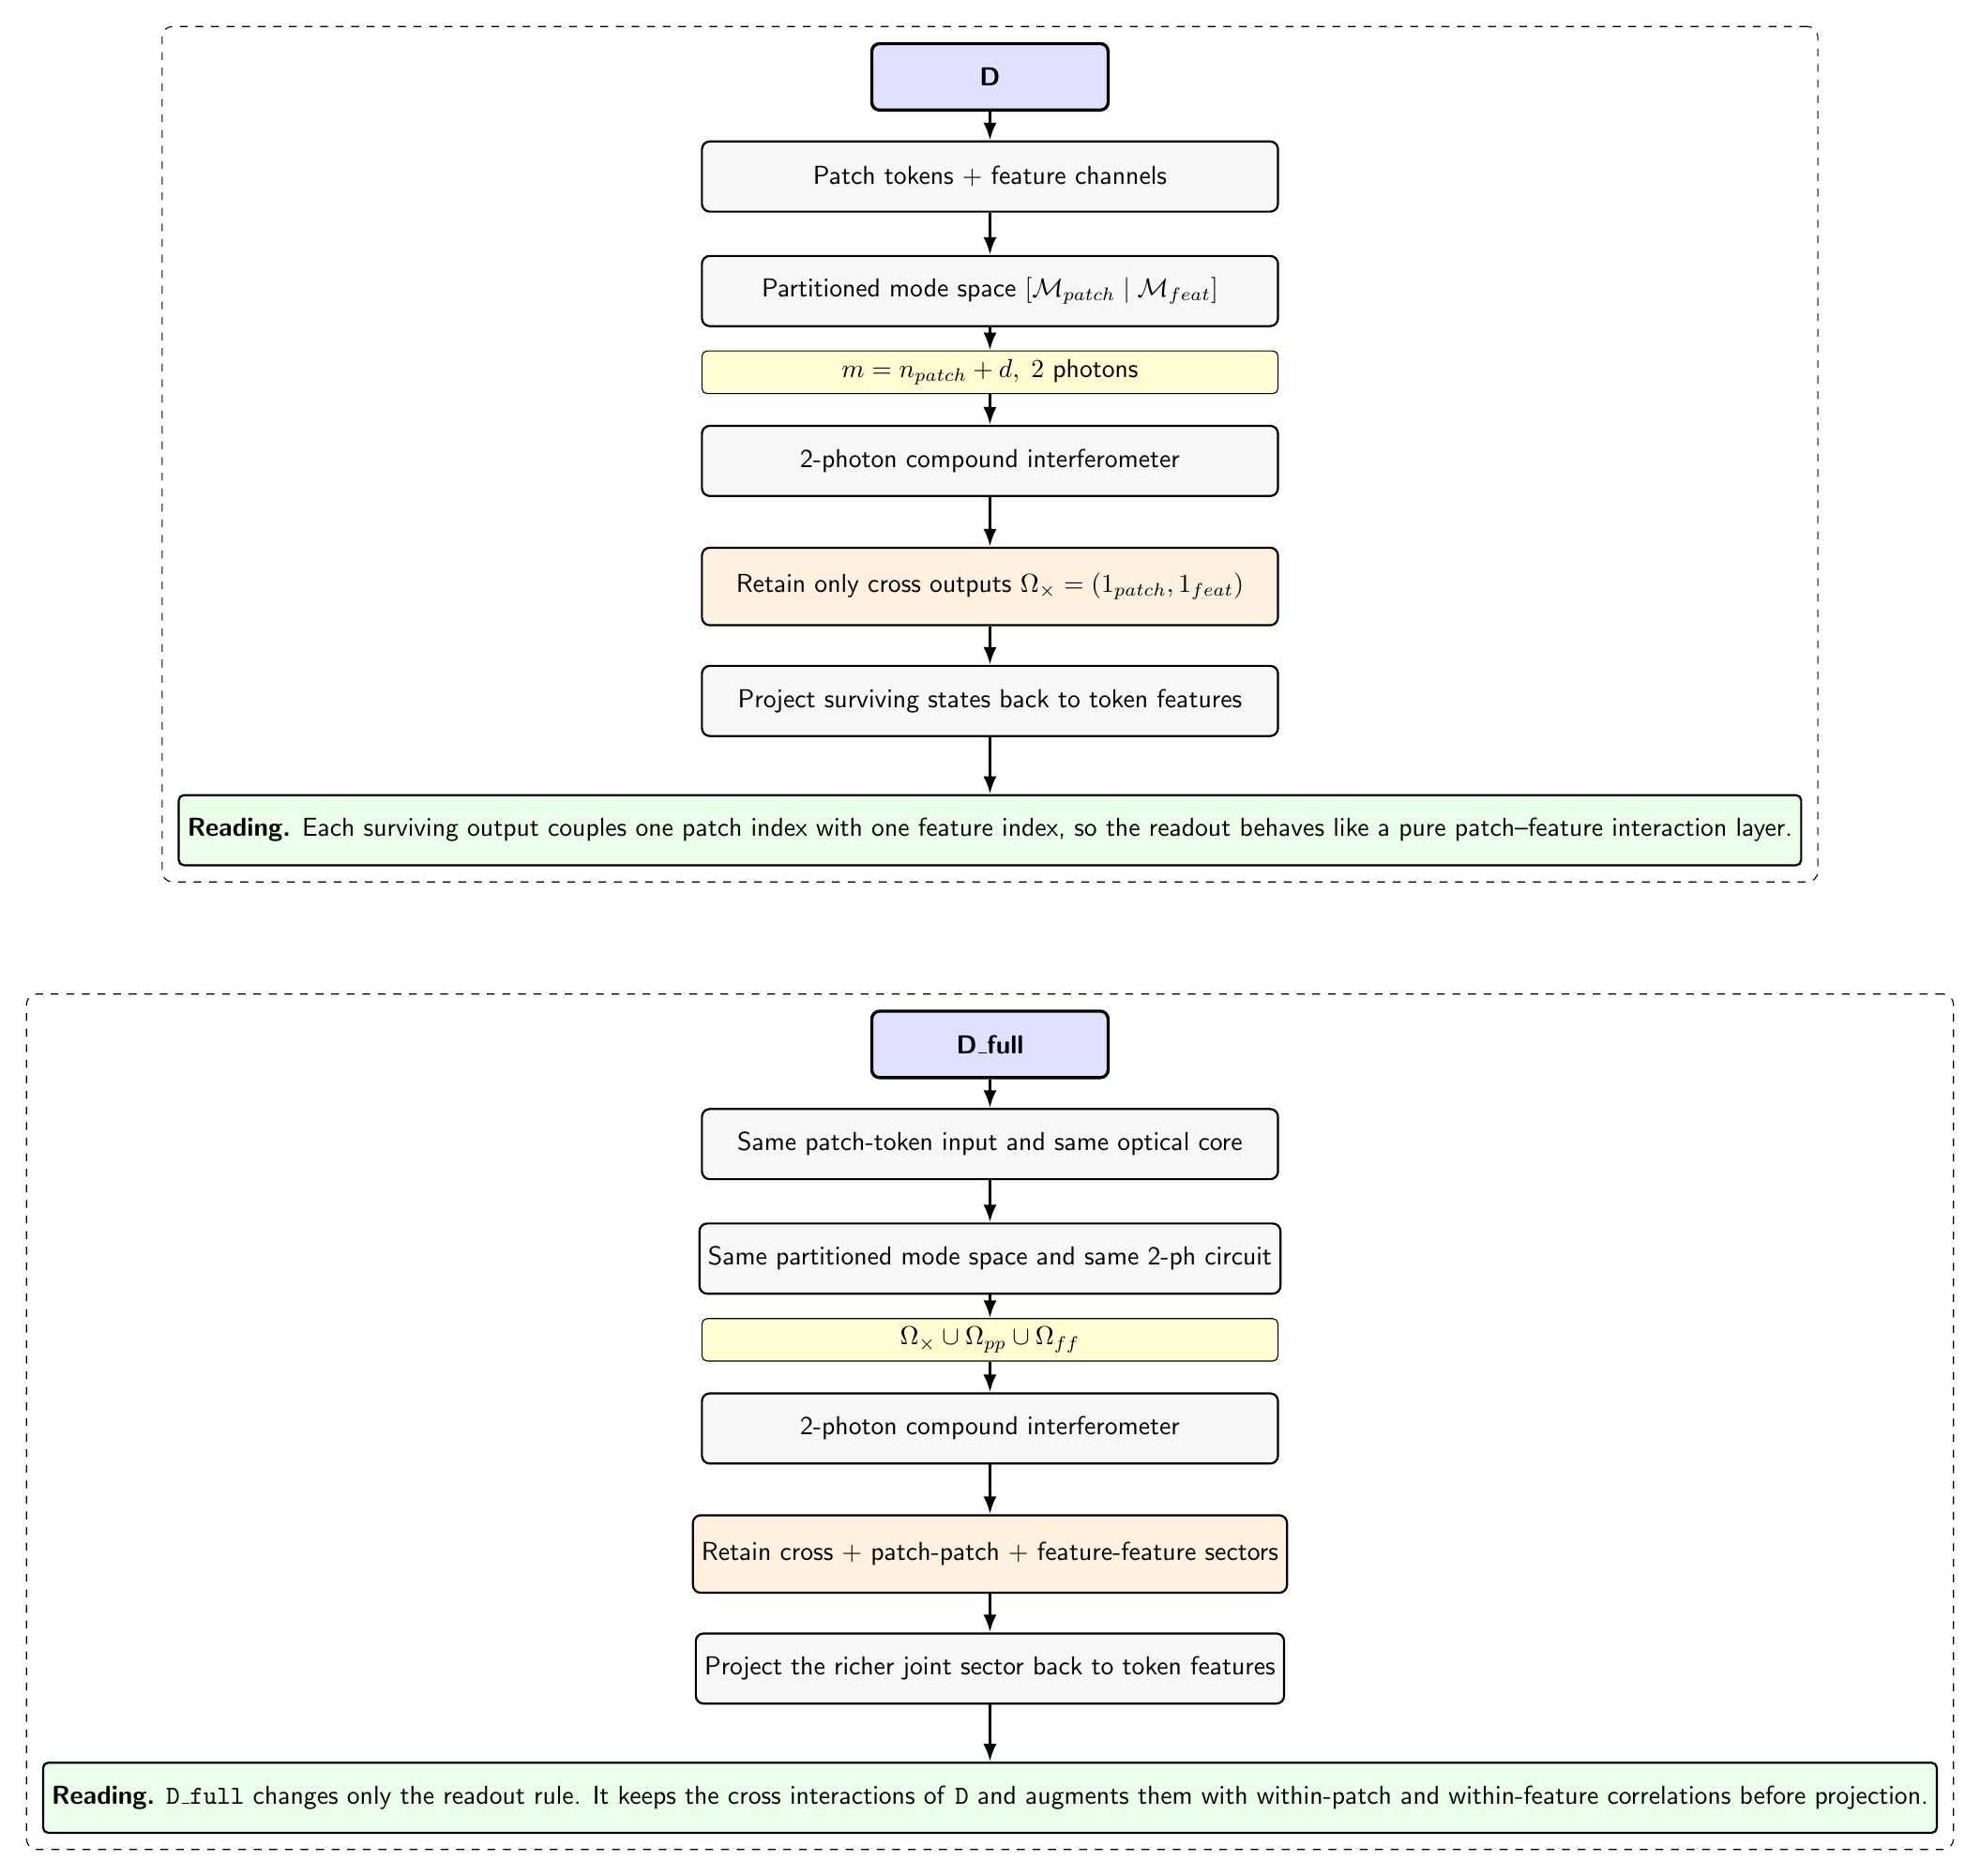
\begin{tikzpicture}[
  font=\sffamily,
  x=1cm, y=1cm,
  title/.style={draw, rounded corners=3pt, minimum width=3.2cm, minimum height=0.9cm, align=center, fill=blue!12, very thick},
  stage/.style={draw, rounded corners=3pt, minimum width=7.8cm, minimum height=0.95cm, align=center, fill=gray!6, thick},
  sector/.style={draw, rounded corners=3pt, minimum width=7.8cm, minimum height=1.05cm, align=center, fill=orange!12, thick},
  ann/.style={draw, rounded corners=2pt, minimum width=7.8cm, minimum height=0.55cm, align=center, fill=yellow!18, thin},
  note/.style={draw, rounded corners=2pt, minimum width=10.8cm, minimum height=0.95cm, align=left, fill=green!8, thick},
  arrow/.style={-{Latex[length=2.4mm]}, very thick},
  dashedbox/.style={draw, dashed, rounded corners=4pt, inner sep=6pt}
]

% D
\node[title] (dtitle) at (5.5, 0.0) {\textbf{D}};
\node[stage] (d0) at (5.5, -1.35) {Patch tokens + feature channels};
\node[stage] (d1) at (5.5, -2.9) {Partitioned mode space $[\mathcal{M}_{patch}\mid\mathcal{M}_{feat}]$};
\node[ann]   (da1) at (5.5, -4.0) {$m=n_{patch}+d,\;2$ photons};
\node[stage] (d2) at (5.5, -5.2) {2-photon compound interferometer};
\node[sector] (d3) at (5.5, -6.9) {Retain only cross outputs $\Omega_{\times}=(1_{patch},1_{feat})$};
\node[stage] (d4) at (5.5, -8.45) {Project surviving states back to token features};
\node[note]  (dn) at (5.5, -10.2) {\textbf{Reading.} Each surviving output couples one patch index with one feature index, so the readout behaves like a pure patch--feature interaction layer.};

% D_full
\node[title] (ftitle) at (5.5, -13.1) {\textbf{D\_full}};
\node[stage] (f0) at (5.5, -14.45) {Same patch-token input and same optical core};
\node[stage] (f1) at (5.5, -16.0) {Same partitioned mode space and same 2-ph circuit};
\node[ann]   (fa1) at (5.5, -17.1) {$\Omega_{\times}\cup\Omega_{pp}\cup\Omega_{ff}$};
\node[stage] (f2) at (5.5, -18.3) {2-photon compound interferometer};
\node[sector] (f3) at (5.5, -20.0) {Retain cross + patch-patch + feature-feature sectors};
\node[stage] (f4) at (5.5, -21.55) {Project the richer joint sector back to token features};
\node[note]  (fn) at (5.5, -23.3) {\textbf{Reading.} \texttt{D\_full} changes only the readout rule. It keeps the cross interactions of \texttt{D} and augments them with within-patch and within-feature correlations before projection.};

\draw[arrow] (dtitle.south) -- (d0.north);
\draw[arrow] (d0.south) -- (d1.north);
\draw[arrow] (d1.south) -- (da1.north);
\draw[arrow] (da1.south) -- (d2.north);
\draw[arrow] (d2.south) -- (d3.north);
\draw[arrow] (d3.south) -- (d4.north);
\draw[arrow] (d4.south) -- (dn.north);

\draw[arrow] (ftitle.south) -- (f0.north);
\draw[arrow] (f0.south) -- (f1.north);
\draw[arrow] (f1.south) -- (fa1.north);
\draw[arrow] (fa1.south) -- (f2.north);
\draw[arrow] (f2.south) -- (f3.north);
\draw[arrow] (f3.south) -- (f4.north);
\draw[arrow] (f4.south) -- (fn.north);

\begin{scope}[on background layer]
  \node[dashedbox, fit=(dtitle) (dn)] {};
  \node[dashedbox, fit=(ftitle) (fn)] {};
\end{scope}
\end{tikzpicture}
\end{document}
